\chapter{Introducción Específica} % Main chapter title

\label{Chapter2}

%----------------------------------------------------------------------------------------
%	SECTION 1
%----------------------------------------------------------------------------------------

El presente capítulo presenta los requerimientos del dispositivo, una descripción de los bloques que lo componen y la planificación que se siguió para lograr satisfactoriamente el desarrollo.

%----------------------------------------------------------------------------------------

\section{Requerimientos}

El dispositivo tiene dos tipos de requerimientos, funcionales y no funcionales. Los funcionales, se refieren a la capacidad para cumplir con ciertas tareas impuestas, que garantizan un correcto desempeño del dispositivo en general. Los no funcionales, tienen relación con temas de carácter económico e informativo.

\subsection{Requerimientos funcionales}

\begin{itemize}
	\item El dispositivo deberá poseer conexión Wi-Fi\footnote{Wi-Fi. Es una tecnología inalámbrica para la interconexión de dispositivos electrónicos.}
	\item El dispositivo deberá funcionar como servidor web local.
	\item El dispositivo deberá contar con la hora y fecha exactas.
	\item El dispositivo deberá interpretar los pulsos ópticos provenientes de un medidor de consumo de energía eléctrica domiciliario.
	\item El dispositivo deberá poseer una memoria no volátil para registrar datos como la hora, fecha, conteo de pulsos e ID del usuario; durante al menos tres meses.
	\item El dispositivo deberá contar con un sistema de adquisición, procesamiento, transmisión y recepción de datos, el mismo podrá ser implementado en un microcontrolador con Wi-Fi integrado.
	\item El dispositivo deberá poseer una interfaz web para que los usuarios puedan observar un registro histórico de su consumo de energía eléctrica.
	\item El dispositivo deberá poder establecer conexión con un gateway LoRa, para enviar diariamente en formato hexadecimal la hora, fecha, consumo de energía eléctrica e ID del usuario.
\end{itemize}

\subsection{Requerimientos no funcionales}

\begin{itemize}
	\item El dispositivo deberá tener un precio menor a 50 \$us.
	\item El dispositivo deberá contar con manuales de uso e instalación.
\end{itemize}

%----------------------------------------------------------------------------------------

\section{Esquema general del sistema}

Para cumplir con todos los requerimientos funcionales expuestos en la sección anterior, los componentes mínimos necesarios y su interconexión se muestran en el diagrama en bloques de la figura 2.1.

\begin{figure}[h]
	\centering
	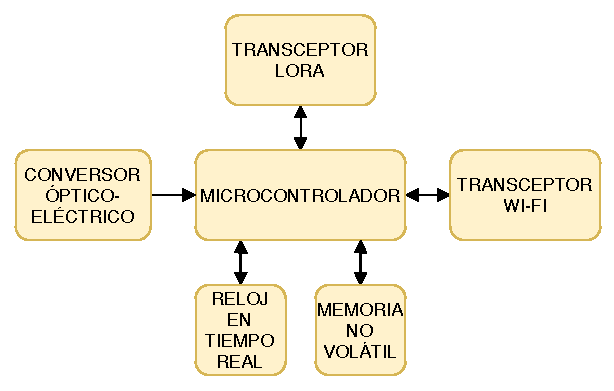
\includegraphics[scale=1.2]{./Figures/general_blocks.pdf}
	\caption{Diagrama en bloques general del dispositivo.}
	\label{fig:cuadradoAzul}
\end{figure}

En el diagrama anterior, el conversor óptico-eléctrico transforma pulsos ópticos a eléctricos y los entrega al microcontrolador con transceptor Wi-Fi. Los pulsos junto con la fecha proveída por el reloj en tiempo real, son almacenados en la memoria no volátil. El transceptor LoRa, se utiliza para transmitir los datos almacenados en la memoria no volátil y recibir información de otros dispositivos conectados a la red LoRa. Por último, el microcontrolador con transceptor Wi-Fi, implementa un servidor web local para que mediante una interfaz gráfica se puedan conocer los datos almacenados en la memoria no volátil.

\subsection{Conversor óptico-eléctrico}

Es el encargado de convertir la salida de pulso óptico de medidores eléctricos digitales a pulsos eléctricos, para que puedan ser interpretados por un microcontrolador. Esta información determina el consumo eléctrico que registra el medidor.

La salida de pulso óptico de los medidores eléctricos digitales, esta compuesta por un LED de color rojo, que emite luz cuando se ha consumido una cierta cantidad de kWh. El valor de la relación entre los pulsos emitidos y el consumo eléctrico, es un parámetro intrínseco del medidor, que varía según el modelo y la firma que lo fabrica.

Para realizar la conversión de pulsos de luz a pulsos eléctricos, existen principalmente dos transductores que cumplen cabalmente esta función:

\begin{itemize}
	\item Fotoresistencia: es una resistencia cuyo valor se modifica en función a la intensidad de luz incidente. También es conocida como LDR (\textit{Light-Dependent Resistor}, resistencia dependiente de la luz) \citep{BOOK:2}. En la figura 2.2 se observa una fotoresistencia.
	
	\begin{figure}[h]
		\centering
		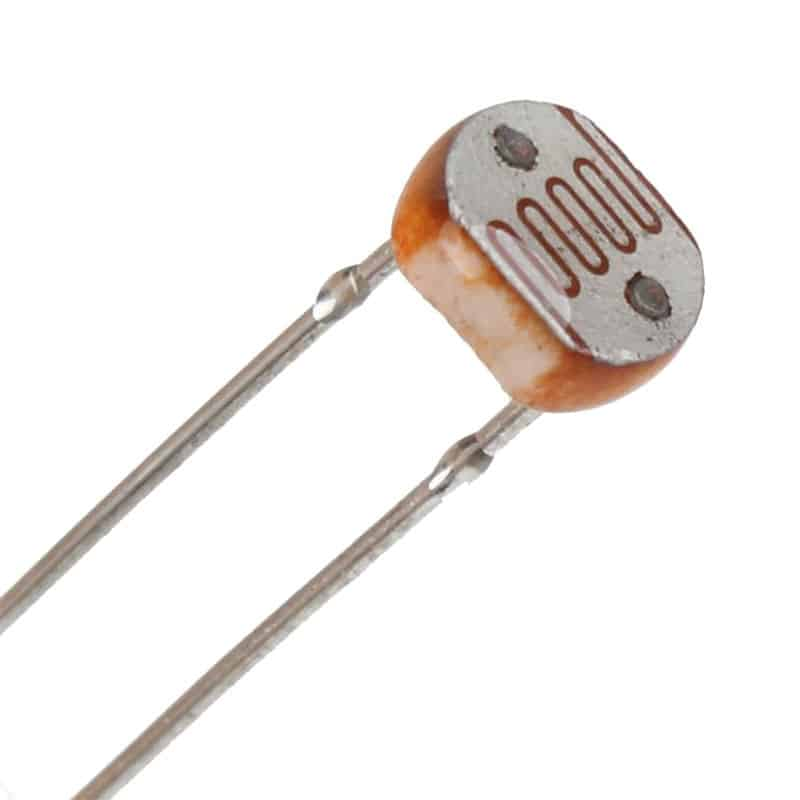
\includegraphics[scale=0.15]{./Figures/ldr.jpg}
		\caption{Fotoresistencia GL5528.}
		\label{fig:cuadradoAzul}
	\end{figure}
	
	\item Fototransistor: es un transistor sensible a la luz, normalmente a los infrarrojos. La cantidad de luz incidente es proporcional a la corriente de base generada. Generalmente tiene el factor de forma de un LED \citep{BOOK:2}. Un fototransistor de uso común se observa en la figura 2.3.
\end{itemize}

	\begin{figure}[h]
		\centering
		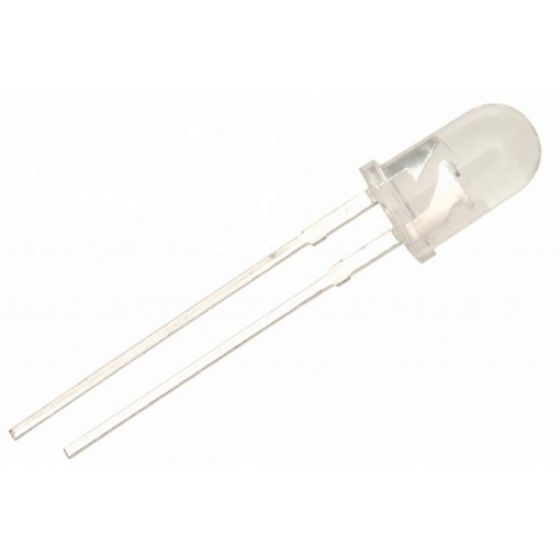
\includegraphics[scale=0.3]{./Figures/phototransistor.jpg}
		\caption{Fototransistor IR333C.}
		\label{fig:cuadradoAzul}
	\end{figure}

\subsection{Microcontrolador con transceptor Wi-Fi}

Este es el componente central del dispositivo. Es el encargado de interactuar con todos los demás bloques, procesar información y proporcionar funciones de redes inalámbricas.

Este tipo de microcontroladores están diseñados principalmente para proveer 

En el mercado, existen una variedad de microcontroladores con \textit{stack} TCP/IP\footnote{TCP/IP. Es un grupo de protocolos  que respaldan a Internet y definen cómo se realiza la transferencia de datos entre redes de ordenadores} incorporado y conectividad Wi-Fi, pero, desde el año 2014 la firma Espressif Systems con sus SoCs (\textit{System on a Chip}, sistema en chip), ha ganado una gran popularidad dentro del desarrollo de dispositivos que requieren conectividad inalámbrica, bajo costo económico y eficiencia energética \citep{WEBSITE:9}.

Los SoCs de Espressif Systems, junto con sus principales características se presentan en la tabla 2.1.

\begin{table}[h]
	\centering
	\caption[caption corto]{caption largo más descriptivo}
	\begin{tabular}{l c c c c}    
		\toprule
		\textbf{SoC} & \textbf{Núcleos} & \textbf{Pines} & \textbf{RAM (KB)} & \textbf{Flash (MB)} \\
		\midrule
		ESP32-S2 & 10 cm & \$ 6.000 & 2 \\		
		ESP32-S2F	 & 15 cm & \$ 7.000 & 2 \\
		Zebrasoma Xanthurus	 & 12 cm & \$ 6.800 & 2 \\
		\bottomrule
		\hline
	\end{tabular}
	\label{tab:peces}
\end{table}

\subsection{Transceptor LoRa}



\subsection{Reloj en tiempo real}

Más conocido como RTC (\textit{Real-Time Clock}, reloj en tiempo real), es un circuito integrado que tiene la capacidad de llevar con precisión la hora y fecha. Para contar con exactitud los segundos, utiliza un oscilador de cristal de cuarzo de 32.768 kHz, que puede o no estar embebido en el encapsulado del RTC.

La principal aplicación de un RTC es brindar a un sistema electrónico la hora y fecha exactas,  también puede ofrecer otras funciones como alarmas, salidas de reloj de 1 Hz o medición de temperatura.

Algunos RTCs tienen una fuente de poder alternativa basada en baterías, que mantiene funcionando la parte del circuito que lleva la cuenta de la hora y fecha. Esta fuente de tensión normalmente son baterías de litio o supercapacitores\footnote{Supercapacitor. Es un capacitor que tiene valores de capacitancia muy altos, pero valores de voltaje muy bajos.}. Comercialmente un RTC puede adquirirse como parte de un módulo, como el que se ve en la figura 2.4, que tiene instalada la fuente de alimentación alternativa y brinda mayor facilidad para acceder a los pines del circuito integrado.

\begin{figure}[h]
	\centering
	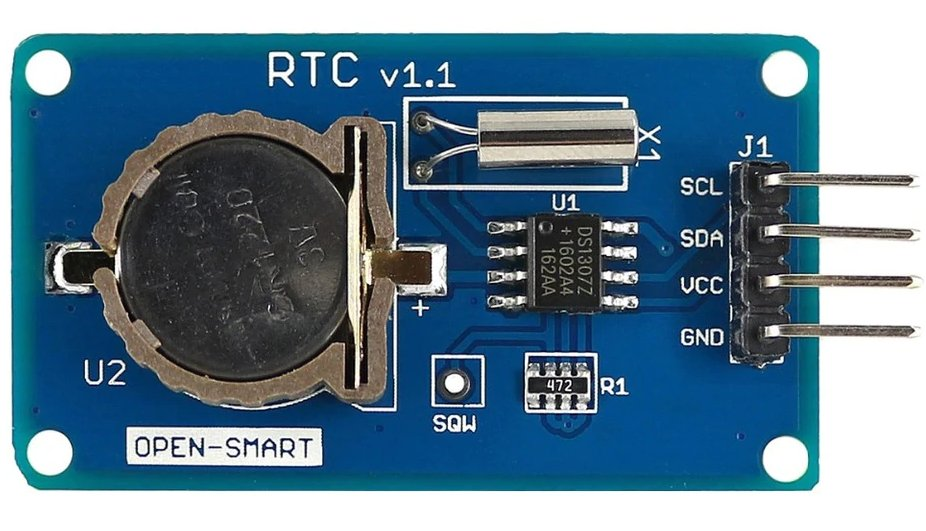
\includegraphics[scale=0.2]{./Figures/rtc.jpg}
	\caption{Módulo RTC basado en el circuito integrado DS1307.}
	\label{fig:cuadradoAzul}
\end{figure}

\subsection{Memoria no volátil}

Es un tipo de memoria de lectura y escritura, en la que los datos que tiene almacenados se mantienen intactos cuando la fuente de alimentación deja de funcionar, es decir, que no necesita energía para mantener guardada la información grabada en ella \citep{BOOK:3}.

En sistemas embebidos, existen principalmente dos tipos de memorias no volátiles:

\begin{itemize}
	\item EEPROM (\textit{Electrically Erasable Programmable Read-Only Memory}, ROM borrable y programable eléctricamente): es un tipo de memoria ROM que puede ser programada y borrada mediante métodos eléctricos. Aunque puede ser leída un número ilimitado de veces, las operaciones de escritura o borrado de datos solo se pueden realizar entre cien mil y un millón de veces. Este tipo de memorias pueden encontrarse como circuitos integrados que generalmente disponen de comunicación I2C o SPI. En la figura 2.5 se aprecia un módulo EEPROM, comercialmente esta es la forma más habitual de encontrarlo.
	\begin{figure}[h]
		\centering
		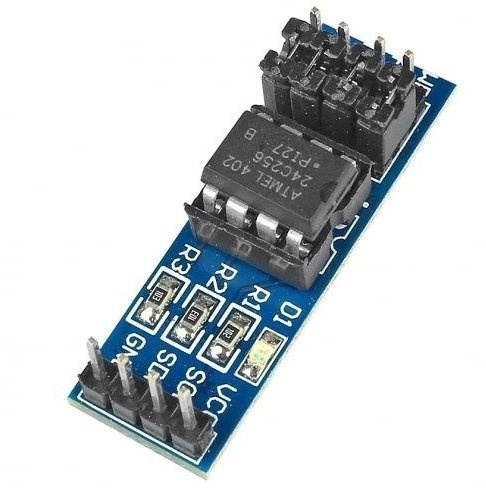
\includegraphics[scale=0.35]{./Figures/eeprom.jpg}
		\caption{Módulo EEPROM basado en el circuito integrado 24C256.}
		\label{fig:cuadradoAzul}
	\end{figure}
	\item Flash: está basada en las memorias EEPROM y permite la lectura y escritura de múltiples posiciones de memoria de manera simultánea, gracias a ello su velocidad de funcionamiento es superior a su antecesor. El número de operaciones de escritura o borrado es de diez mil a un millón. Es empleada principalmente en la fabricación de memorias USB y unidades de estado sólido. Asimismo, los microcontroladores actuales tienen integrada una unidad de memoria flash para el almacenamiento de instrucciones y datos. Para la realización de pruebas y prototipos, existen comercialmente módulos de memoria flash con comunicación SPI, como el de la figura 3.6.
	\begin{figure}[h]
		\centering
		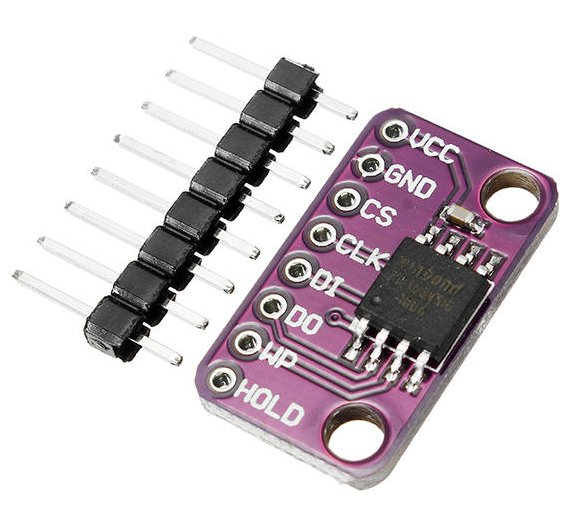
\includegraphics[scale=0.35]{./Figures/flash.jpg}
		\caption{Módulo flash basado en el circuito integrado W25Q16BVSIG.}
		\label{fig:cuadradoAzul}
	\end{figure}
	
\end{itemize}

%----------------------------------------------------------------------------------------

\section{Planificación}

Como se explicó en la subsección 2.2, el dispositivo esta compuesto por diferentes bloques funcionales, que tienen tanto componentes de firmware como de hardware. 

%----------------------------------------------------------------------------------------